% !TEX encoding = UTF-8
% !TEX TS-program = pdflatex
% !TEX root = ../tesi.tex
% !TEX spellcheck = it-IT

%**************************************************************
\chapter{Strumenti e tecnologie utilizzate}
\label{cap:strumenti-tecnologie}
%**************************************************************

Il contenuto di questo capitolo contiene una descrizione più dettagliata delle tecnologie e degli strumenti utilizzati per sviluppare l'applicativo oggetto dello stage.

\section{React Native}
\todo[inline]{Cosa scrivere?}
Come anticipato nel precedente capitolo, si è scelto di utilizzare React Native come framework principale per lo sviluppo dell'applicazione.

\todo[inline]{L'applicazione è composta da componenti (con pattern smart \& Dumb --> ogni componente ha uno stato --> rendering}


\subsection{La sintassi JSX}
\todo[inline]{Parlare di come viene usata per definire il layout dei componenti}

\subsection{Componenti esterni}
\todo[inline]{todo: react-native-popover e react-native-cookies}


\section{Flux}
Flux è un pattern architetturale per le applicazioni sviluppate con React e React Native proposto da Facebook.

Questo pattern sfrutta il sistema di composizione delle view di React costruendo un flusso di dati unidirezionale, che a partire da un oggetto \textit{store} diventano lo stato di un oggetto \textit{view-controller}, che a sua volta li fornisce ai propri componenti.

L'unico modo per modificare i dati presenti in uno \textit{store} è mediante un \textit{action}, quando un \textit{view-controller} vuole modificare i dati a seguito di un evento scatenato dall'utente, crea un \textit{action} che, mediante un \textit{dispatcher}, viene ricevuto dai vari \textit{store} dell'applicazione.

\begin{figure}[htp]
\centering
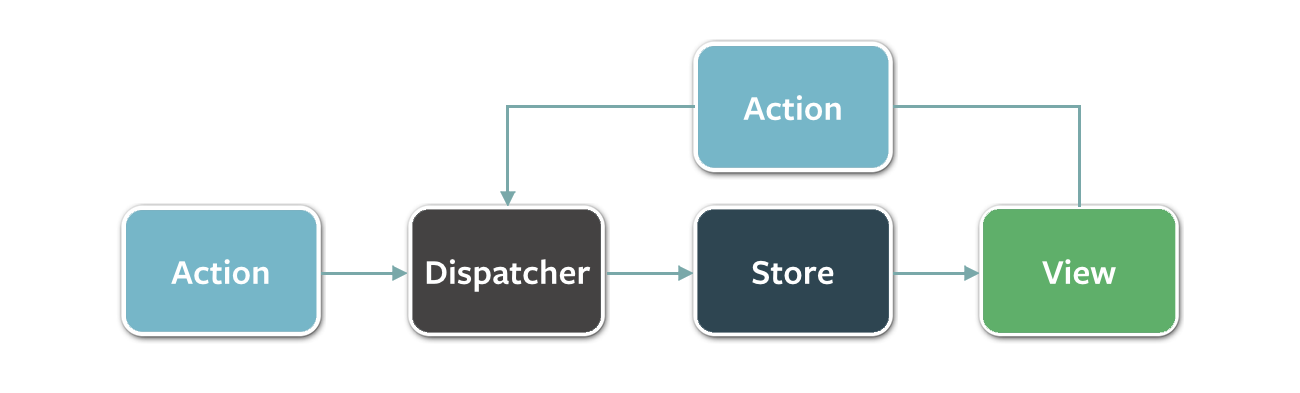
\includegraphics[width=\textwidth*3/4]{../immagini/flux-simple}
\caption{Diagramma del pattern Flux}  
\end{figure}
\FloatBarrier

Come anticipato, Flux prevede tre tipologie principali di componenti:
\begin{itemize}
\item \textbf{Stores:} sono dei \textit{singleton} che contengono i dati dell'applicazione, forniscono solamente dei metodi \textit{getter}, per interagire con i dati contenuti è necessario usare le \textit{actions}.
\item \textbf{Actions:} sono degli oggetti che contengono delle informazioni riguardante alle varie operazioni che possono eseguite dagli \textit{stores} dell'applicazione. Tipicamente vengono create dai \textit{view-controller} di React e contengono già i dati necessari agli \textit{store} per aggiornarsi, nel caso di operazioni asincrone i \textit{view-controller} creano l'azione che verrà comunicata al \textit{dispatcher} solamente quando sono stati caricati i dati.
\item \textbf{Dispatcher:} oggetto che riceve un \textit{action} e ne esegue il broadcast verso tutti gli \textit{stores} registrati dell'applicazione. Fornisce delle funzionalità che permettono ai vari \textit{stores} di registrarsi e di specificare eventuali dipendenze verso altri \textit{stores} dell'applicazione in modo che l'aggiornamento di un determinato \textit{store} venga effettuato una volta completato l'aggiornamento degli \textit{stores} da cui dipende, evitando così di ottenere uno stato inconsistente.
\end{itemize}


\subsection{Sequenza delle azioni}

\begin{figure}[htp]
\centering
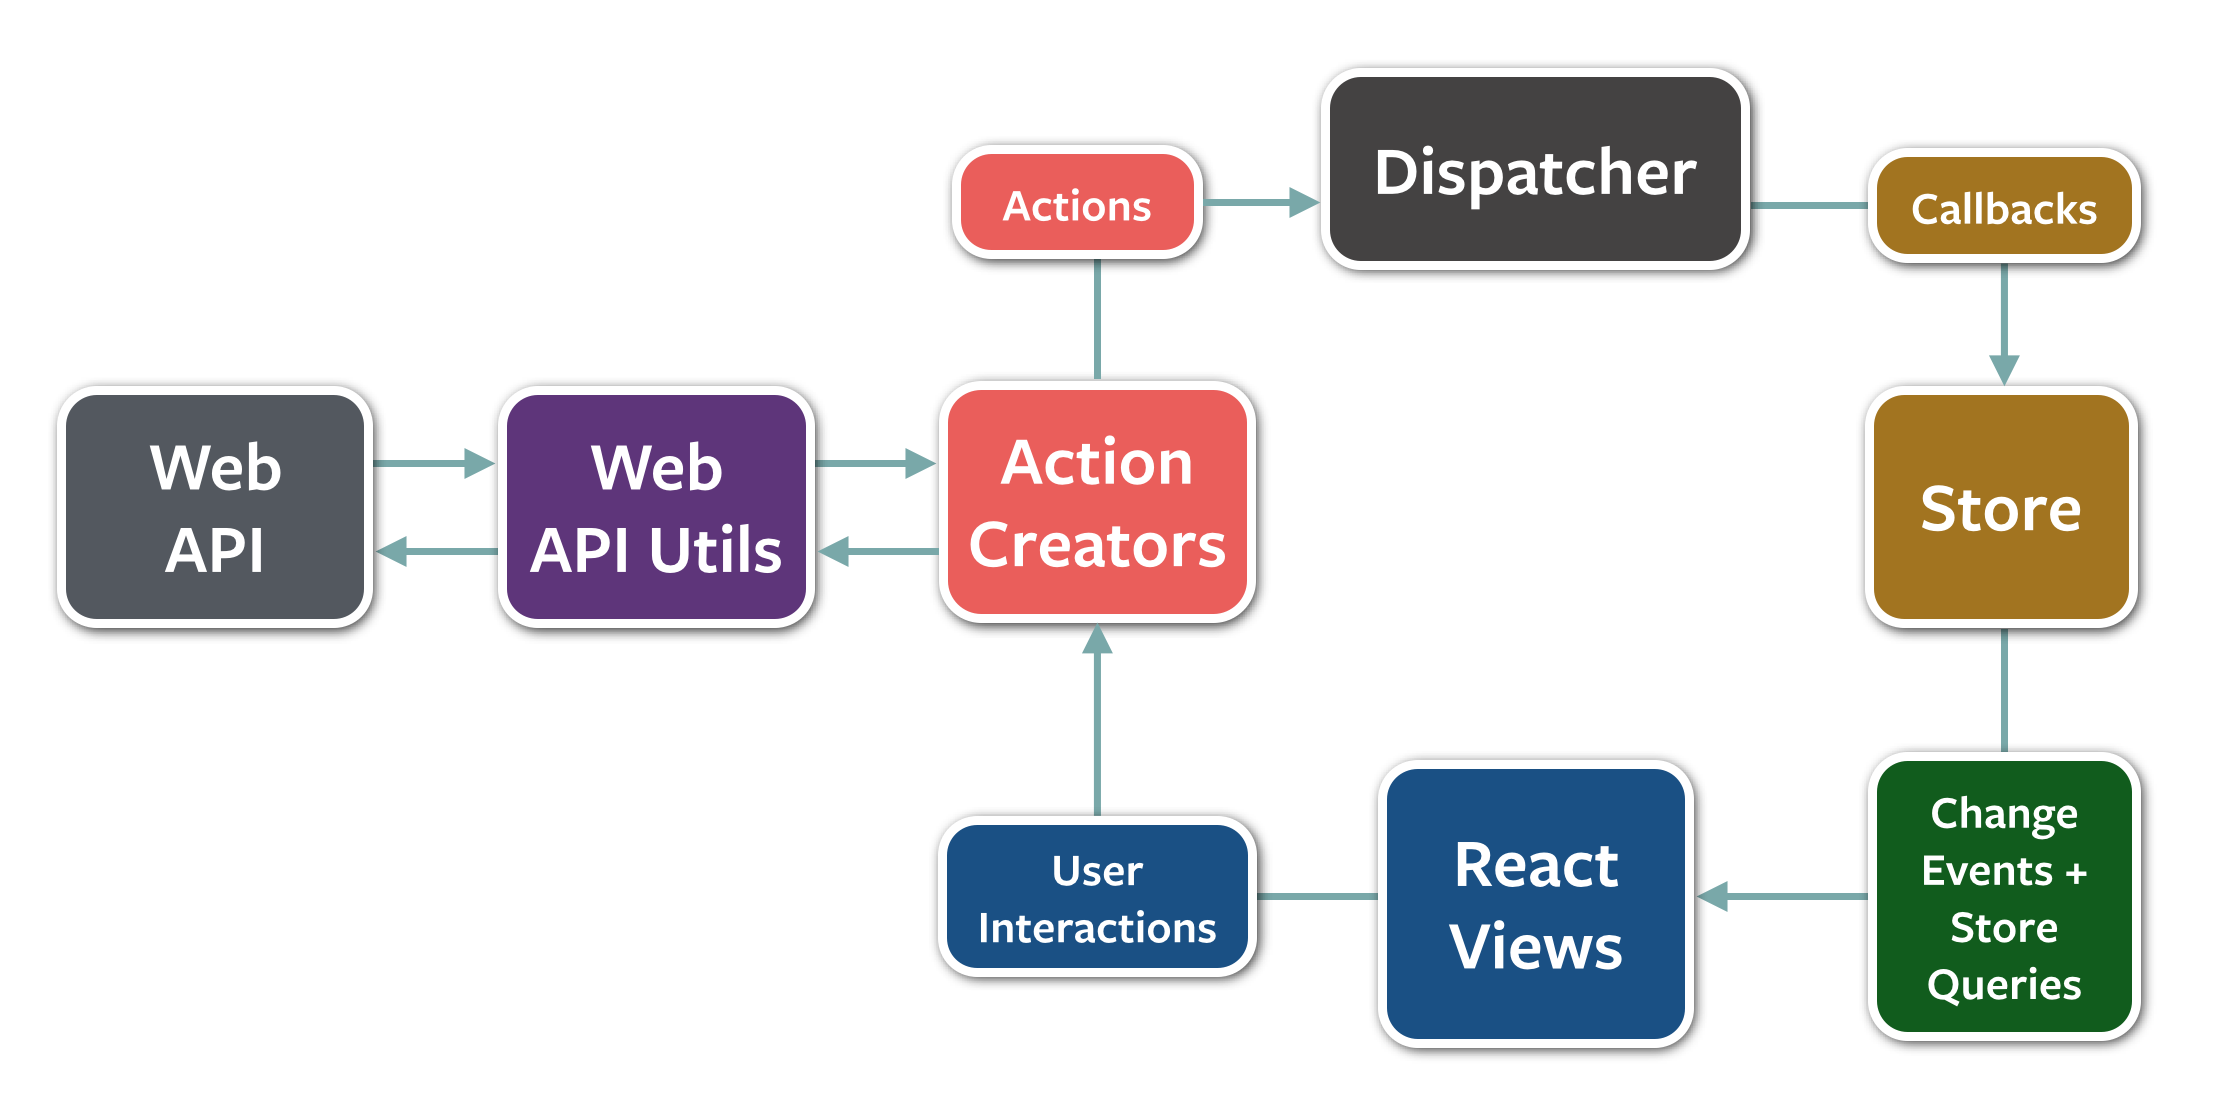
\includegraphics[width=\textwidth*3/4]{../immagini/flux-diagram}
\caption{Funzionamento del pattern Flux}  
\end{figure}
\FloatBarrier

\begin{enumerate}
\item L'utente esegue un'azione sulla view.
\item Il gestore dell'evento crea un \textit{action} e la comunica al \textit{dispatcher}.
\item Il \textit{dispatcher} manda a tutti gli \textit{stores} registrati l'oggetto \textit{action} ricevuto.
\item Ogni \textit{store} esamina l'oggetto  \textit{action} e se necessario si aggiorna. 
\item Gli \textit{stores} che hanno subito modifiche emettono un evento per comunicare ai componenti React in ascolto che si devono aggiornare.
\item I componenti React richiedono agli \textit{stores} i dati per aggiornarsi.
\end{enumerate}

\subsection{Differenze con MVC}

Nonostante Flux ed MVC possano sembrare due pattern totalmente diversi, in realtà Flux è una variante del MVC classico con delle modifiche che lo adattano al funzionamento di React e React Native.

Infatti, con MVC, i \textit{controllers} interagiscono con il \textit{model} e le \textit{view} dell'applicazione visualizzano i dati presenti al suo interno.
Quando il \textit{model} viene modificato, le \textit{view} vengono notificate e recuperano i dati aggiornati dal model.

Mentre con Flux, i \textit{view-controller} aggiornano il model, definito dagli \textit{stores}, in un modo più strutturato utilizzando le \textit{actions} e, una volta che l'aggiornamento degli \textit{store} è completato, i \textit{view-controller} vengono notificati in modo che possano recuperare i nuovi dati.

Considerando che per React e React Native una \textit{view} e il relativo \textit{controller} sono lo stesso oggetto diventa chiaro che la logica di base è la stessa, l'unica differenza è come viene effettuato l'aggiornamento dei dati, che con Flux deve passare attraverso delle \textit{actions}.

Questo vincolo imposto dall'utilizzo delle \textit{actions} permette di circoscrivere la logica di aggiornamento del model all'interno del model stesso, limitando la complessità dell'applicazione, che nel caso di grandi applicazioni può diventare ingestibile.

Un altro vantaggio che viene dall'adozione di Flux con React riguarda l'aggiornamento dell'interfaccia grafica a seguito di una modifica dei dati, in quanto sia React che Flux ragionano a stati: con React l'interfaccia grafica visualizza uno stato dell'applicazione, il cambiamento dello stato comporta il re-rendering dell'interfaccia, mentre con Flux l'insieme degli \textit{stores} rappresenta lo stato dell'applicazione e l'esecuzione di un'azione comporta il cambiamento dello stato.

Di conseguenza è possibile collegare direttamente lo stato definito dagli \textit{stores}, con lo stato dei componenti grafici, limitando il numero di operazioni intermedie.

\section{Flow (?)}








